% !TEX root = QlockToo.tex

\section{Konstruktion und Produktion}
\label{sec:KonstruktionFertigung}

\begin{multicols}{2}
Um die Herstellungskosten möglichst gering zu halten wird die ClockToo als eine Kombination aus Kaufteilen und eigener Produktion ausgeführt. Ziel ist eine möglichst getreue Nachbildung der Original CLOCKTWO® der Biegert~\&~Funk Manufacture GmbH \& Co. KG. 

\textbf{Das Uhrgehäuse}

Die Basis für das Uhrengehäuse bildet der IKEA-Bilderrahmen RIBBA in schwarz. Die Bilddarstellungsmaße von 50 x 50 cm eigenen sich gut, um die Buchstabenmatrix zur Geltung zu bringen. 

{
\centering 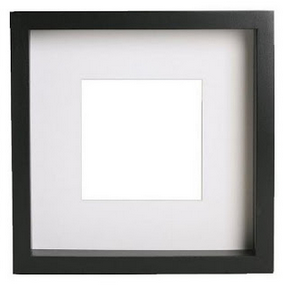
\includegraphics[width=0.75\columnwidth]{Abbildungen/Konstruktion/Ribba02} %Bilderrahmen

}
In dem besonders tiefen Rahmen,  Tiefe~=~4,5~cm, kann die komplette LED-Matrix inklusive der Elektronik untergebracht werden. Lediglich zum Hinausführen des Stromkabels und zur Anbringung der Taster muss der Rahmen leicht modifiziert werden.


\textbf{Buchstabenfolie}

Zur Darstellung der Zeit in Worten wird eine schwarze Folie mit einer negativen Buchstabenmatrix auf eine Plexiglasscheibe geklebt. Die Anordnung der Buchstaben entspricht der Original CLOCKTWO®. 

{
\centering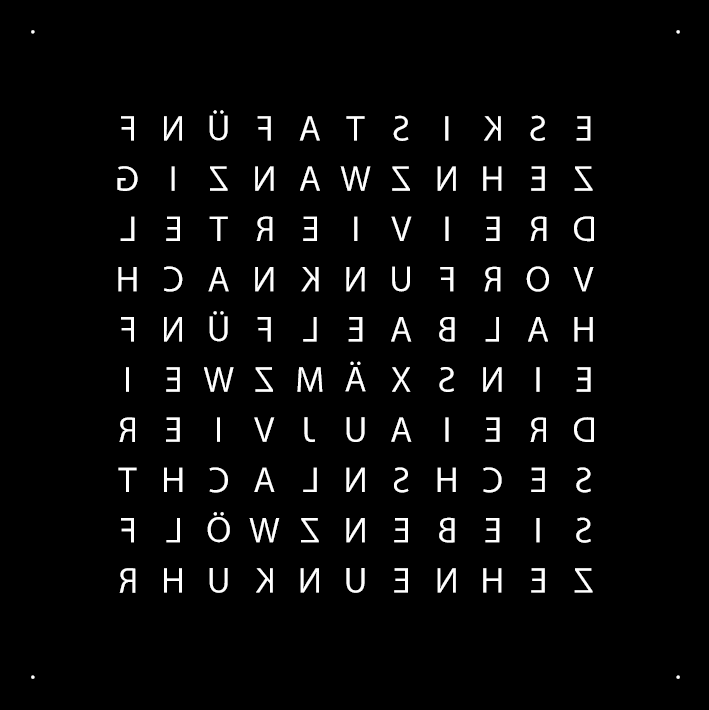
\includegraphics[width=0.75\columnwidth]{Abbildungen/Konstruktion/Buchstaben}

}
Mit der gewählten Buchstabenmatrix ist die Uhr auf eine deutsche Anzeige festgelegt. Die Original CLOCKTWO® CLASSIC beherrscht zwölf Sprachen. Durch Austauschen des Frontcovers kann die gewünschte Sprache eingestellt werden. 

\textbf{LED-Matrix}

Die LED-Matrix wird aus einer quadratischen Spanplatte gefertigt. Abbildung ~\ref{fig:Spanplatte} zeigt die Fertigungs- bzw. Bearbeitungszeichnung der Spanplatte. Diese wird entsprechend der vorgegebenen Buchstabenmatrix -  10~x~11 Buchstaben - gebohrt und gesenkt, sodass die LEDs die kompletten Buchstaben ausleuchten können. 

{
\centering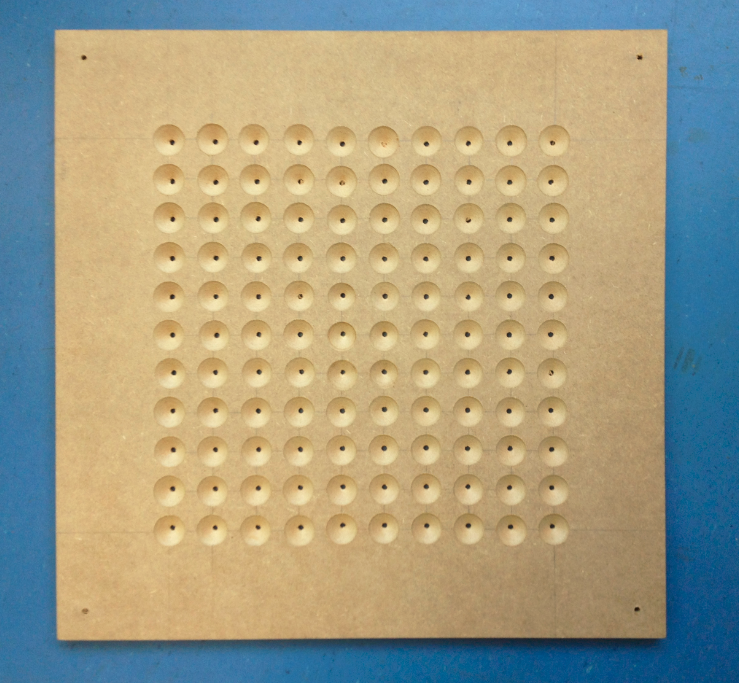
\includegraphics[width=0.85\columnwidth]{Abbildungen/Konstruktion/Platte01}

}
Für den Lichtsensor und für die Minuten-LEDs werden weitere Löcher am oberen Rand und in den vier Ecken gebohrt. Zusätzlich wird ein Ausschnitt zur Aufnahme der Platine aus der Platte gefräst. 

{
\centering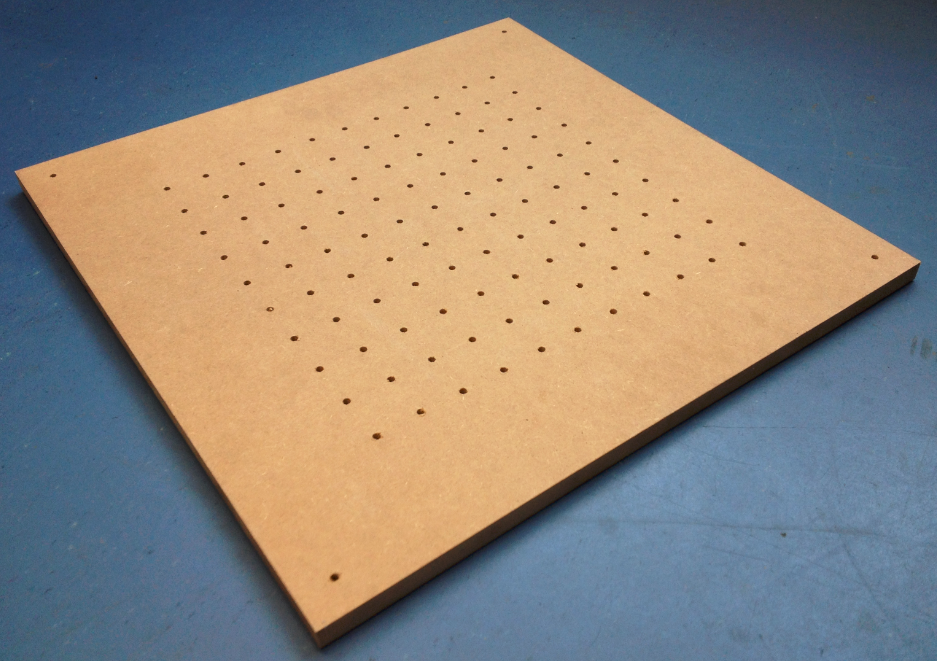
\includegraphics[width=0.85\columnwidth]{Abbildungen/Konstruktion/Platte02}

}
Die LEDs werden entsprechend hinter den Löchern positioniert, verdrahtet und mit Heißkleber fixiert. 

{
\centering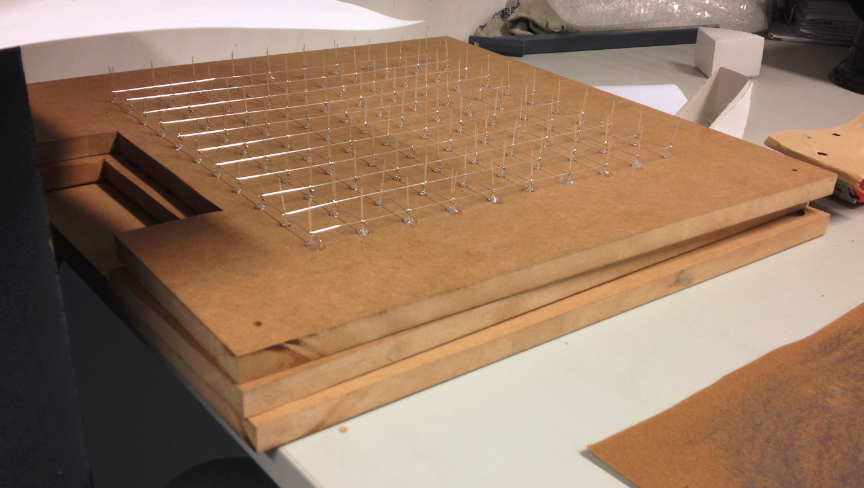
\includegraphics[width=0.85\columnwidth]{Abbildungen/Konstruktion/LED01}

}
Ohne eine zusätzliche Streuung kann man die LEDs hinter den jeweiligen Buchstaben deutlich erkennen. Eine vollständige Ausleuchtung ist in dieser Phase nicht möglich. 

{
\centering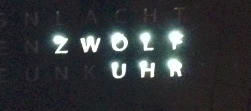
\includegraphics[width=0.85\columnwidth]{Abbildungen/Konstruktion/LED03}

}
Um eine möglichst breite Streuung des LED-Lichtes zu erzielen, wird hinter die Buchstabenfolie eine zweite Diffusorfolie  geklebt. Trotz der doppelten Folie ist die Streuung des Lichtes nicht ausreichend. Um diese zusätzlich zu erhöhen, wird ein Streuplättchen (D:~25~mm) aus transparentem Papier in die gesenkten Kegel geklebt. 

{
\centering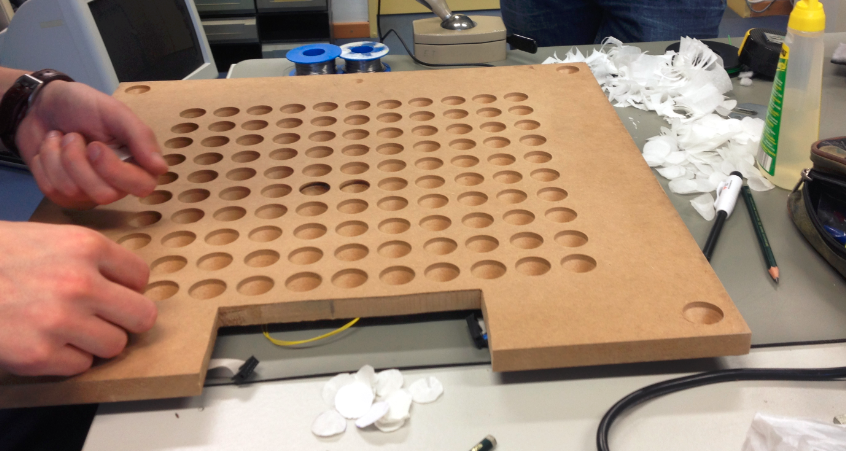
\includegraphics[width=0.85\columnwidth]{Abbildungen/Konstruktion/LED02}

}



\end{multicols}

\begin{landscape}
	\begin{figure}
		\centering
		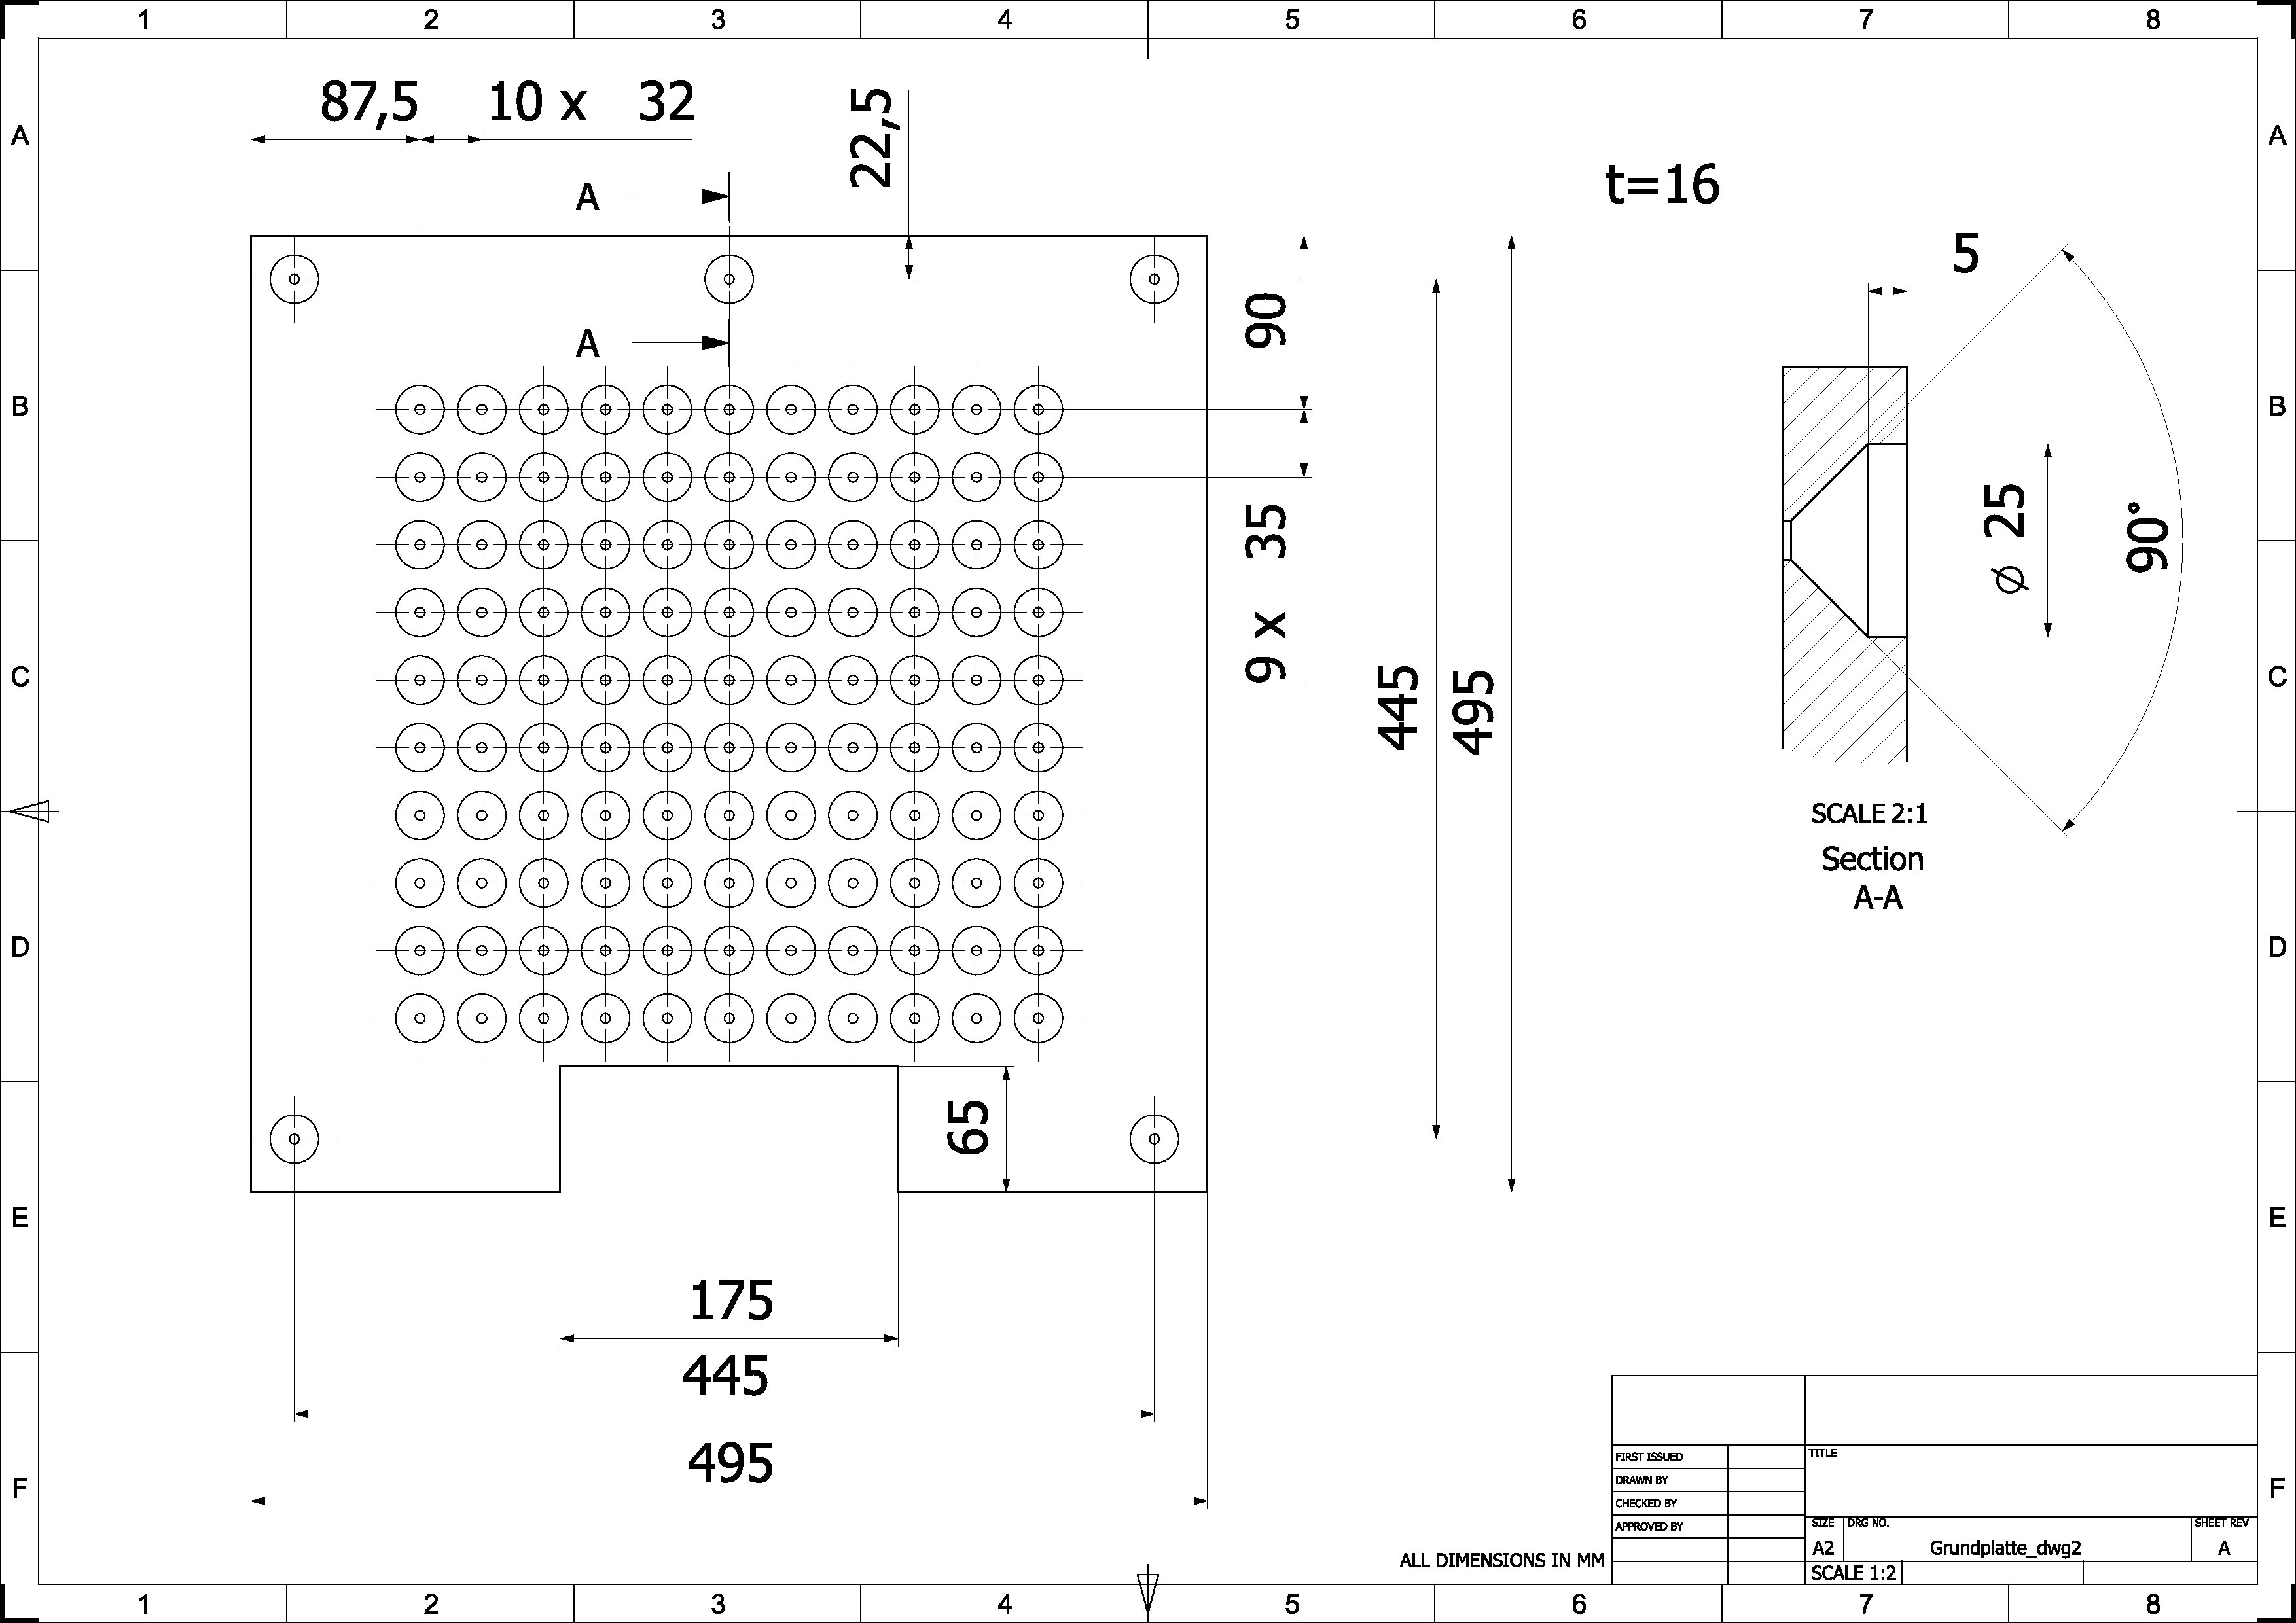
\includegraphics[width=21cm]{Abbildungen/Konstruktion/Grundplatte}
		\caption[Spanplatte]{Fertigungszeichnung Spanplatte}
		\label{fig:Spanplatte}
	\end{figure}
\end{landscape}


